\section{Sistema de Comunicación Humano-Máquina (S6)}
La implementación del sistema de comunicación humano-máquina se realizó apegándose a la arquitectura definida en la fase de diseño, integrando un módulo de visualización física para entradas y salidas, y un módulo lógico de gestión de datos. La interfaz actúa como el puente intercambiando información con el sistema de control. A continuación se describe la implementación de los módulos que conforman este sistema.

\subsection{Implementación del módulo E/S (M10)}

El módulo de Entrada/Salida se implementó mediante la integración de hardware de visualización y el desarrollo de una aplicación gráfica de escritorio.

\subsubsection{Integración de Hardware}
Se instaló una pantalla táctil de 7 pulgadas (modelo Waveshare HDMI LCD) montada sobre una carcasa impresa en 3D acoplada a la estructura principal. La conexión con la unidad de procesamiento (Raspberry Pi 4) se estableció mediante:
\begin{itemize}
	\item \textbf{Puerto HDMI:} Para la transmisión de video en alta resolución (1024x600).
	\item \textbf{Puerto USB:} Para la transmisión de datos de la interfaz táctil capacitiva y alimentación.
\end{itemize}

\subsubsection{Desarrollo de Software (GUI)}
La lógica de interacción se programó en lenguaje \textbf{Python 3}, utilizando la librería \textbf{PyQt5} para la construcción de la interfaz gráfica. A diferencia de soluciones básicas, el uso de \textit{Qt Framework} permitió implementar una arquitectura multihilo (\textit{Multithreading}):
\begin{itemize}
	\item \textbf{Hilo principal (Main Thread):} Gestiona los eventos de la interfaz (botones, cambio de ventanas) garantizando una respuesta visual fluida.
	\item \textbf{Hilos de trabajo (Worker Threads):} Se implementaron clases dedicadas (\texttt{QThread}) para ejecutar los bucles de control de los motores y la lectura de sensores mediante la librería \texttt{pigpio}. Esto evita que la interfaz se congele durante la ejecución de las rutinas de terapia.
\end{itemize}
La navegación se estructuró mediante un \texttt{QStackedWidget} que administra las pantallas de: \textit{Inicio, Posicionamiento inicial, Calibración, Selección de Terapia, Pantalla de ejercicio y Ejecución}\footnote{El código fuente completo de la aplicación, incluyendo la interfaz gráfica, se encuentra disponible en el repositorio público del proyecto: \url{https://github.com/ramsalue/ortesis-robotica}}.
\begin{figure}[h!]
	\centering
	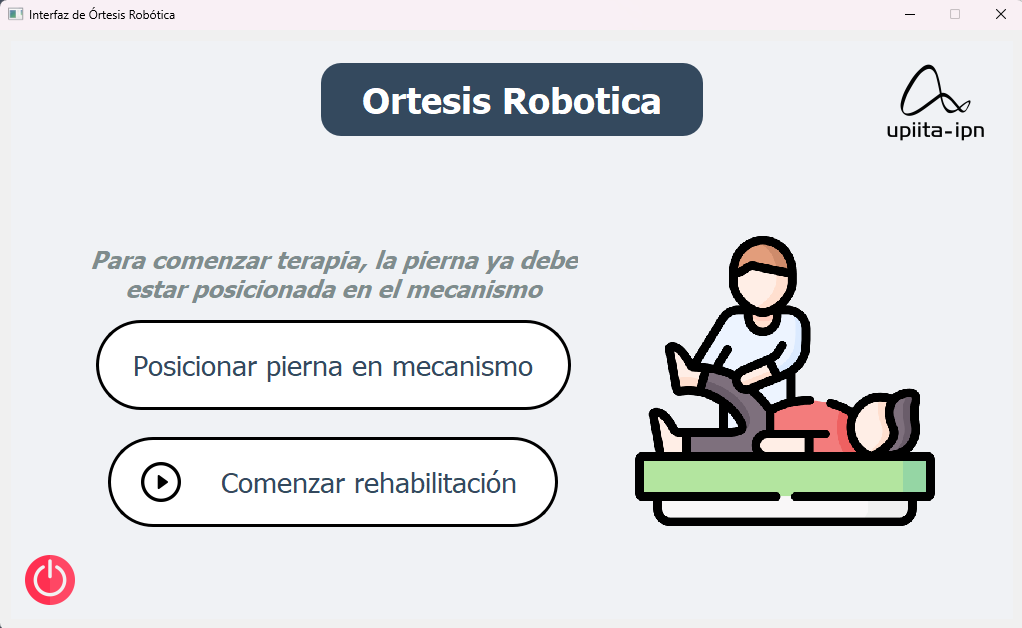
\includegraphics[width=0.48\textwidth]{figure/pantallas_interfaz/App Ver1.0/Inicio_tt2.png}
	\hfill
	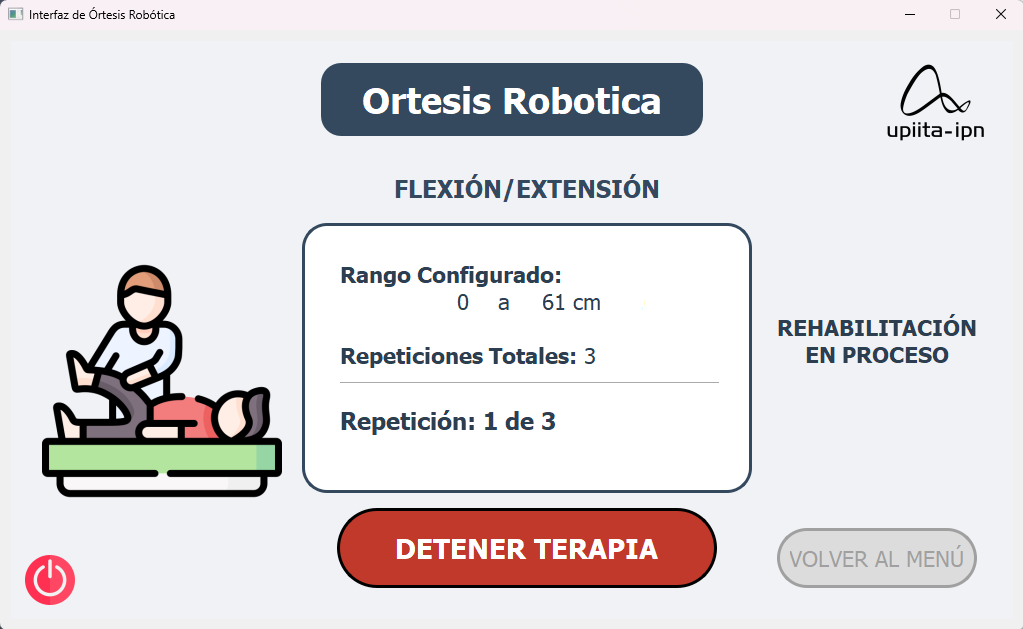
\includegraphics[width=0.48\textwidth]{figure/pantallas_interfaz/App Ver1.0/Terapia_tt2.png}
	\caption{Interfaz gráfica implementada: Pantalla de Bienvenida (izq) y Monitor de Terapia (der).}
	\label{fig:gui_screens}
\end{figure}
\vspace{-0.5cm}
\subsubsection{Verificación del módulo E/S}
\paragraph*{Prueba S6-01: Respuesta táctil y fluidez gráfica.}\mbox{}\\
\textbf{Objetivo:} Verificar que la interfaz responde a los eventos táctiles en tiempo real y se ajusta a la resolución nativa sin distorsión.
\\
\textbf{Procedimiento:} Se ejecutó el script \texttt{app\_fisioterapia.py} en el entorno real. Se realizaron pulsaciones rápidas en los botones de navegación y se observó el consumo de CPU.
\\
\textbf{Resultados:} La interfaz ocupa la totalidad del área activa (Fullscreen). La transición entre menús es menor a 100ms. Los botones táctiles activan correctamente las señales lógicas sin necesidad de teclado/mouse externo.

\subsection{Implementación del módulo de almacenamiento (M11)}

Este módulo, encargado de alojar el sistema operativo, los scripts de control y los recursos gráficos (imágenes), se implementó sobre un medio de almacenamiento de estado sólido.

\subsubsection{Configuración del sistema de archivos}
Se utilizó una tarjeta MicroSD de 32GB (Clase 10 / UHS-I) para conseguir altas velocidades de lectura/escritura, que son importantes para el arranque del sistema operativo Raspberry Pi OS.
La estructura de directorios se organizó para permitir el acceso relativo a los recursos, independientemente de la ruta absoluta de instalación:
\begin{verbatim}
	/home/pi/TT2_Software/
	├── app_fisioterapia.py   (Código fuente principal)
	├── styles.py            (Hoja de estilos y constantes visuales)
	└── icons/              (Iconos, logotipos y diagramas de ayuda)
\end{verbatim}

Esta organización permite que el software sea portable y facilita la actualización de los archivos de imagen sin modificar el código fuente.

\subsubsection{Verificación del módulo de almacenamiento}
\paragraph*{Prueba S6-02: Integridad de recursos y persistencia.}\mbox{}\\
\textbf{Objetivo:} Confirmar que el sistema puede leer correctamente los archivos almacenados en el módulo M11 durante la ejecución.
\\
\textbf{Procedimiento:} Se inició la aplicación y se navegó a la pantalla de "Selección de Ejercicio", la cual requiere cargar dinámicamente imágenes explicativas desde la carpeta \texttt{assets}.
\\
\textbf{Resultados:} Todas las imágenes se renderizaron correctamente. El sistema operativo arrancó y ejecutó el script de autorun sin errores de "File Not Found", validando la integridad del sistema de archivos implementado.